\section{Prototype Analysis} \label{sec:prototype_analysis}
As this thesis builds upon the PowerPedia prototype, it is appropriate to analyze its functionality and technical realization in detail. This analysis serves as the bases to draw conclusions about the further development of the platform. 

PowerPedia can be accessed in two ways so far. Users can brows through its content using the web interface or the Android eMeter application, which communicates directly with the platform and integrates its functionality. The web user interface allows users to brows through PowerPedia's data using a standard web browser.
%This consideration makes it important to analyze its functionality and to a lesser degree, its technical realization and current status as well.
     
%Both the web platform and the mobile phone application were build for research purposes and could not be accessed publicly (TODO: is that so?). 

\subsection{Functionality}
\subsubsection{Web platform}
PowerPedia's main functionality is storing and managing measurements conducted by users with an eMeter mobile phone client. 
The purpose behind collecting this data is to be able to determine the energy efficiency of devices by comparing them to other devices of the same device category. As a secondary feature, PowerPedia collects electricity saving tips and tricks proposed by its users.

In particular the detailed functionalities of the PowerPedia web platform are as follows:

\minisec{Storage of measurements}
In order to determine the energy efficiency of an appliance, it is essential to know the energy consumption of other, comparable devices. These consumption values can either originate from an external source as described below in TODO or they can come from other users. In both cases, the data needs to be saved and organized somewhere. Thus, the PowerPedia prototype is mainly a central server for storing measurement data. 

\minisec{Device management}
Every measurement is linked to an electric appliance. Whenever users upload measurements to PowerPedia, the device that was measured needs to be specified as well. Devices can be created by users or they can be extracted from the measurement data that comes from external sources. PowerPedia manages and stores those devices.  

\minisec{Category management}
Knowing the energy consumption of a device is not enough to compare the device to others. It is also important to categorize appliances such that only the ones in the same category are compared to each other to get reasonable results. Moreover, categories are a way of organizing devices that are stored on the platform. PowerPedia uses a hierarchical scheme for device categories, where categories can have subcategories. Every device is assigned to exactly one category. 

\minisec{Device ranking calculations}
A ranking can be computed for every device that is published on PowerPedia. Within the device's category, all devices are sorted according to their energy consumption. The ranking consists of multiple parts. The device's position in this list is one, the total number of devices in the category another. Also, it includes the consumption value of the best and the wort device of the category. Moreover, the value is compared to the values of the best and worst device and visualized with an icon with four bars of different colors to give the user a quick overview whether this device is closer to the worst or the best device in its category. 

\minisec{Energy conservation tips}
Users can share their energy conservation tips on PowerPedia. Tips have a category, which has a name, a description, and an URL that links to the source of the tips.
		 
\minisec{User management}
PowerPedia's user management is mainly for the web user interface. 
Apart from the tips functionality, its content is only accessible for registered users. Users have to create an account and provide their username and password to see the restricted content. 
Logged in users can get an overview of all the devices they uploaded as well as their published measurements. A measurement linked to a device and a user is called a "Recognition" on PowerPedia.\todo{is that in fact so?}
  
\minisec{Harvester}
The Harvester module of PowerPedia fetches data from external webpages to initialize and update the device database. Initially, it fills the database with values to enable the rating of devices, which depends on comparative data. When updating the device list, most recent data is considered and the database is kept up to date. 
%The prototype uses the Swiss consumer webpage Topten.ch\footnote{http://www.topten.ch/}, from where it also adapts the device category structure. 

\minisec{HTML representation}
\begin{figure}[htbp]
\begin{center}
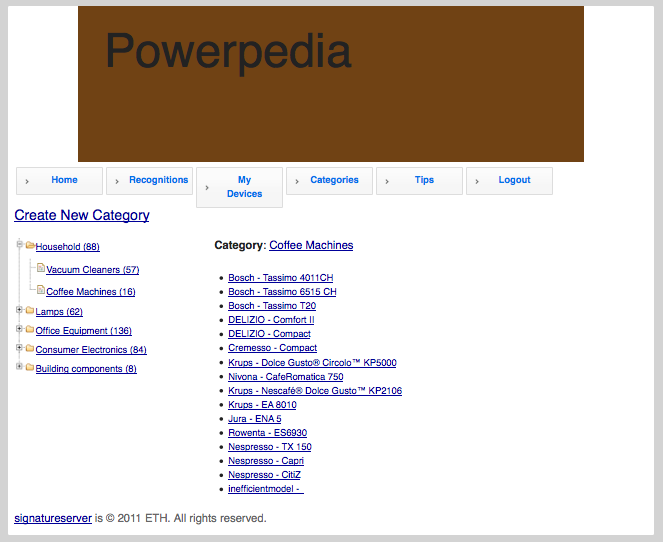
\includegraphics[width=13cm]{Images/pp.png}
\caption{PowerPedia web user interface, category section}
\label{pp}
\end{center}
\end{figure} 
PowerPedia offers a human readable representation of its data. It allows users to navigate through the device categories and to view the uploaded data using a web browser.

The HTML representation has following parts:
\begin{description}
\item[Login] On the login page, users can register for the system. Username, password, first and last name are required values users have to provide. Registered users can log into the system with their username and password. 
\item[Home] In the Home section, personal information of the user are displayed and can be edited. 
\item[Recognitions] All the uploaded measurements (recognitions, measurements linked to a device and user) of the user are listed in this section. For each recognition, there is a link to the corresponding device that was measured.
\item[My Devices] My devices includes all devices the user has published. Each device has a link to its category and detail page, which displays further information such as manufacturer, image, and ranking information.
\item[Categories] Categories are displayed hierarchically. When clicking on categories that contain no further subcategories, a list with all devices of that category is displayed (see figure~/ref{pp}). 
\item[Tips] In the tips section, energy saving tips can be found. They are grouped in categories, which have a name, description and URL that points to the source. 
\item[Logout] The user is logged out of the system and redirected to the login screen.
\end{description}

\subsubsection{Mobile phone application}
\missingfigure{include screenshots?}

As the original mobile phone client for the iPhone, the Android eMeter application communicates with the energy server to get data collected by the smart electricity meter. Communication with PowerPedia is new and so far only supported by the Android user interface.
 
Following functionality (that is relevant for PowerPedia) was introduced in the Android application:

\minisec{Device categorization}
Due to the fact that PowerPedia works with device categories, users can now assign categories to devices on the mobile phone client. Users can select from categories fetched from PowerPedia.

\minisec{Measurement and device upload}
When a user measures the energy consumption of a device with the Android mobile phone application, he can choose to publish the measurement on PowerPedia. Since PowerPedia needs to know the associated device, the user has two options. If the device already exists in PowerPedia's device database, the user can assign the measurement to this existing device. In order to do so, he first selects the corresponding category (and subcategories, if applicable) and then the device from lists fetched from PowerPedia.
If no matching device can be found on the platform, the user has to provide the details himself. The newly created device can then be upload to the platform as well.  
 
\minisec{Device rating}
Devices for which the user has made measurements have a detail view. This view includes information such as manufacturer and image if available, but also the device's rating as calculated by PowerPedia.  

\minisec{Tips checklist}
The Android eMeter application also includes a new main view that doesn't exist on the iPhone application: the Tips view. Tips are displayed as a checklist, where users can check tips they have already completed. More tips can be loaded from PowerPedia. So far, a hard coded list with tips is used initially. 

\subsection{Technical Details}
\subsubsection{Web platform}
As described earlier, in order to be able to compare devices, measurement data needs to be stored on a central instance. This central instance, in this case PowerPedia, needs to be accessible via both a web interface and mobile phone clients. To achieve this goal, PowerPedia had to be designed in a modular way. Above all, design and architectural decisions had to consider this requirement.

\minisec{Design decisions}
The PowerPedia web platform was implemented in PHP using the Recess\footnote{\url{http://www.recessframework.org/}} framework, version 0.20. Several platform alternatives were considered, namely using a Wiki, implementing a Facebook application, or building the entire system from scratch with a web application framework. For various reasons, the decision felt on the last option and on Recess. 
One of the advantages of Recess is its support for REST (for details on REST, refer to section TODO). This feature makes developing modular applications easy.

Finding an appropriate web technology for a productive version of PowerPedia is a concern of this thesis as well. Section~\ref{TODO} illustrates various technologies, their advantages and disadvantages, and reasons for choosing Recess in detail.  
  
\minisec{Architecture}
\missingfigure{Figure similar like in~\cite{weiss:inprocPUC:2012}}
PowerPedia is primarily the backend to store data that is created by users when they conduct a measurement on the mobile phone client. In figure TODO, the architecture of of PowerPedia and its position in the overall eMeter infrastructure is depicted. The system consists of three main components: the SignatureServer that stores device data, the harvester module that automatically updates the system with the newest device information, and the user interface. So far, there are two user interfaces, an Android and a web interface. 

The System can be installed on any apache server\footnote{\url{http://www.apache.org/}}. Because every component of the eMeter system uses TCP/IP connections for all communications, components can communicate with each other over the internet, over a local network, or they can even reside on the same machine.

Data on PowerPedia is stored in a MySQL database\footnote{\url{http://www.mysql.com/}}. The database can be accessed using PDO\footnote{PDO stands for "PHP Data Objects". It defines a lightweight and consistent interface for accessing databases\cite{merklepp}.}

In terms of software architecture, the platform follows the REST\cite{Fielding2000} and Movel-View-Controller (MVC)\footnote{The original implementation is described in~\cite{burbeck87}} principles. Both concepts are encouraged by the Recess framework. Recess has build-in support for REST, which enablers users to access PowerPedia's API using URIs\footnote{Unified Resource Identifiers (URIs) are strings that identify resources in the web \url{http://www.w3.org/Addressing/}}\cite{weiss:inprocPUC:2012}. 
%The usual HTTP verbs GET, PUT, POST, and DELETE can be used to access and manipulate resources. Also, REST is very flexible in terms of data representation. By specifying the relevant file extensions (.html for HTML or .json for JSON), the corresponding data formats 
 
\missingfigure{include figure similar to Figure 5.3: Powerpedia object model, page 51}

Recess also already uses a loosely coupled Model-View-Controller architecture.
Figure TODO depicts the resource model of PowerPedia. Because of the importance of comparing devices, the recognition model is central to the system. It defines the interface clients have to use to publish electricity consumption measurements on PowerPedia. A recognition needs to be linked to both a registered user and a device, include a start and end date, and specify the watt values measured at the start date and the end date. Furthermore, it has a creation timestamp.

\minisec{Harvester}
The harvester's purpose is to fetch data from external webpages and extract their energy efficiency information. This data is parsed from the HTML documents of those pages and then stored in the PowerPedia device database.
There are several webpages that offer a comparison between devices in the same category. Topten.ch \footnote{\url{http://www.topten.ch/}} is the site that has been chosen because it proved to be an ideal candidate. According to their international website, Topten is a "search tool, which presents the best appliances in various categories of products"\footnote{\url{http://www.topten.info/english/services/about_topten.html}, accessed in September 2011}. The site was launched in Switzerland in 2000 and has been growing and expanding ever since to seventeen other countries. 

For every new external webpage, the harvester has to be extended due to the individual layout and structure of websites. So far, the harvester is only configured for Topten.ch. A monthly cron job on the host initiates the fetching process. HTML documents are parsed and scanned for category and device information. 

The harvester is implemented in PHP. Since all communication with PowerPedia is done over the internet, the harvester module does not have to reside on the same host as PowerPedia. 

\todo{is that detailed enough?}

\minisec{Rating algorithm}
Rating devices is one of the main features of PowerPedia, which makes it necessary to take a closer loot at the underlying algorithm.
In order to be able to rate the consumption of a device against the devices in the same category, it's consumption in watt and it's category id must be available. 
The rating information consists of \textit{count}, \textit{position}, \textit{best}, \textit{worst}, \textit{rating}. The position is determined by sorting all devices in the category, where the \textit{position} then denotes the number of devices that consume less energy. \textit{Best} and \textit{worst} are the watt values of the best and worst device in the category. The rating is a number between 0 and 3. Figure TODO shows how this number is determined.
\missingfigure{Figure: worst --- +25\% | 1 --- +50\% | 2 --- +75\% | 3 --- best}
 
\subsubsection{Mobile phone application}
\minisec{Design decisions}
The Android eMeter application was developed with Android 2.1 with the Java programming language\footnote{\url{http://java.com/}}.

Prior to~\cite{merklepp}, the only user interface to access the energy server was the iPhone eMeter client. To make the eMeter system available to a broader set of users, the functionality of the iPhone application was ported to the Android operating system. Android has become a popular operating system for mobile phones and smart phones running on it a considerable alternative for the iPhone.

\minisec{Architecture}   
Communication with the web platform is the aspect of the Android eMeter client that is relevant for this work. The application communicates with PowerPedia in two ways, on one hand, it fetches data such as tips and device categories, on the other, it uploads data such as measurements and new devices.  

Because PowerPedia is RESTful, the application can interact with the data on the platform by using URIs over the internet. Thus, in able to communicate with PowerPedia, standard Java http packages can be used\todo{is that correct?}. Of course, a working internet connection is needed.

\subsection{Development stage and reusability}
\todo{what does really work on the mobile phone client (loading tips, uploading devices etc.)?}

Developing the PowerPedia web platform was only one part of the earlier mentioned Master thesis. The main focus of that work was on the Android application, which was finalized to such a degree that it could be released to the public \todo{is this correct?}. As one can see in figure~\ref{pp}, especially the web user interface part of PowerPedia is still in an early development stage and can be considered a prototype. Furthermore, the platforms functionality is rather limited. Features were developed around the idea of proving users with device ratings on the mobile phone client. The data model of the application is reasonable and can be reused. 

Because of the Android application's maturity, it makes sense to adopt as much of the platforms functionality as possible. Ideally, the Android mobile phone client can stay the way it is right now with only minor modifications. The communication between clients and PowerPedia is done over the internet using URIs, which would suggest to keep the REST architecture and the routes used so far to access resources.

In terms of code, arguments for evolving the prototype into a productive system or rewriting the entire platform can be found in section~\ref{TODO}\todo{In section about which platform/framwork is used for new version. Evolutionary vs. Throw-Away prototype}. 
The harvester module has a special role in this discussion. Although it is part of the PowerPedia system, it is an independent module that doesn't even have to reside on the same host. All communication is done over the internet. The harvester fills and updates the device database, which it can do without affecting the rest of the system\todo{is that in fact true?}. This process has been tested and works well with the consumer webpage Topten.ch. It can thus certainly be reused in a new system.   

\subsection{Discussion}
\minisec{Use case}
One of the major issues with PowerPedia is its use case. It has to be investigated further what the main use case of this platform is, as this is not inherently clear. As mentioned before, according to PowerPedia's documentation, the main purpose it is to be a central storage point for consumption measurement data. These consumption values are used to enable users to "receive a rating for their device based on other devices already published within the same device-category."\cite{merklepp}. This mainly seems to be valid for users who upload data with the Android eMeter application. When a measurement is performed, in addition to the consumption in watt, users also get back the rating information to better understand the efficiency of the device. 
Because of this rating, it might turn out that the corresponding device is an inefficient device relative to similar devices. Unfortunately, the user already owns it. The usage of such knowledge has to be analyzed further.

For users who access the platform via the web user interface, getting ratings for devices is not so easy anymore. It is also not obvious that this is the main use case for the platform. There is no "Energy efficiency ratings" section, no direct possibility to compare devices in terms of their energy usage. Recognitions can be created by hand, but this process is not very user friendly yet. The user has to manually fill in the device id, a value which is internal to the system. After having entered a recogintion, the device with this id gets a rating.  
In the current development stage of the platform, there is no adequate justification yet why there is a need for a web interface. Also, it it not completely obvious what the user can do with the knowledge that there are better fridges on the market than his fridge, for example.

\minisec{Definition of a measurement}
Collecting measurements on a central server to derive further information from them seems to be a reasonable idea, but unfortunately, exactly the concept of measurements is not trivial. What exactly is measured?    
There are various ways how to conduct those measurements with either the Android or the iPhone eMeter client. The setup largely depends on the device category of the appliance under test, a fact that has not yet been considered. Just to give two examples, how does one measure the consumption of a water cooker? Is switching it on and then off again after a couple of seconds sufficient to determine its electricity consumption? Does every water cooker have the same approach to heating water so that it suffices to stop after a couple of seconds? What about fridges? A fridge does not cool down all the time. Thus, are two measurements, one conducted when the fridge was cooling and one when it wasn't, comparable? 
The eMeter system gives users the possibility to measure the consumption of a device themselves. 
%Because the system can not determine automatically (yet) what kind of appliance is being tested, the measurement largely depends on the set up the user choses (TODO: is that so?).
The resulting value largely depends on the set up the user choses. This might be adequate for devices such as light bulbs, but completely unpredictable for the above mentioned examples. 
With these considerations, it seems necessary to further define measurements. 

\minisec{Tips functionality}
So far, the tips functionality is rather limited. In~\cite{merklepp}, it is differentiated between tip categories and tips in general. Via the web user interface, it is only possible to create categories, but it doesn't seem to be possible to create actual tips. Instead, tip categories link to external sources that contain energy saving ideas. 
 
\minisec{User management}
PowerPedia's user management is quite restrictive. Non-registered users are only allowed to see tips section. Sections of general interest such as categories or home should be accessible publicly. 

\minisec{User interface}
There are several issues with the user interface of the prototype, which would have to be reassessed in a version that is intended for productive use.
\begin{description}
 \item[Main Navigation] The PowerPedia prototype has following navigation items: Home, Recognitions, My Devices, Categories, Logout. This main navigation can be accessed from every page. There is no distinction between logged in and non-logged in users, both user groups see the same categories, although the latter group is redirected to the login page when trying to access a category other than tips. Also, "Logout" looks like an actual navigation category, but it's behavior is like the one of a button. It doesn't have its own page and only results in the user being logged out.
 \item[Home] The home page is the login page at the same time. There is no description about PowerPedia or any other content commonly found on home pages.
 \item[Difference between private and public data] In the "Recognitions" sections, it is not clear whether all recognitions or only the recognitions of the currently logged in user can be found here. The navigation item "My devices" suggests that this section contains only devices the user has created or published. Moreover, the distinction between private data and data that can be accessed by all (logged in or non-registered) users should be clearer. 
 \item[Categories] The concept of categories and devices are mixed. Categories are grouped hierarchically, actual devices of the system form the leaves of the tree. Categories is the only starting point to get to the device database, although this is an important concept of the system.
 \item[Authorization] Every user has the rights to edit or delete devices in "Categories" and tips on the "Tips" page.
\end{description}
The first impression of a webpage is very important for its success. When users are dissatisfied with the navigation, layout or structure of a page, they might not use it again. Providing a useful service is important, but design aspects are of considerable importance as well.	







